\documentclass[10pt]{article}
\usepackage{NotesTeX} %/Path/to/package should be replaced with package location
\usepackage{lipsum}
\usepackage{tensor}
\usepackage{amsmath,amsthm,amssymb}
\usepackage{hyperref}
\usepackage{physics}
\input{undertilde}


\newcommand{\bs}{\textbackslash}


\title{{\Huge General Relativity}\\{\Large{Class  18 - March 3, 2020}}} %replace with class number
\author{Sarah Racz}

\emailAdd{racz.sarah@utexas.edu} %replace with your email
\begin{document}
    \maketitle
    \flushbottom
    \newpage
    \pagestyle{fancynotes}
    %\part{HELLO \LaTeX\,}
	%Use the uncompiled version of this document in itself as a \LaTeX\, style guide for the class you'll be responsible for.
	
	\section{Covariant Derivative Again}
	Last lecture we built the covariant derivative by hand by demanding it met certain conditions. These conditions allowed us to uniquely define a covariant derivative that produces a new tensor when acting on a tensor field. In particular we defined it's action on a vector as 
	\begin{align}
            \nabla_{\mu} T^{\nu} = \partial_{\mu} V^{\nu} + \Gamma^{\nu}_{\mu \alpha} V^{\alpha}.
            \end{align}
            
           Our connection defined uniquely and known as the \textbf{Levi-Civita} connection. 
            
            Recall that he torsion free requirement of the connection gives us that 
            \begin{align}
            \Gamma^{\rho}_{\left[ \mu \nu \right] } = 0 \implies \Gamma^{\rho}_{( \mu \nu ) }  = \Gamma^{\rho}_{ \mu \nu } ,
            \end{align}
            
            which left us with 4 degrees of freedom from $\rho$ and 10 from $\mu \nu$ for a total 40 $\Gamma$s to be determined. We further constrained this by demanding metric compatibility. 
            \begin{align}
            \nabla_\mu g_{\nu \rho} = 0 = \partial_\mu g_{\nu \rho}  - \Gamma^{\alpha}_{\mu \nu} g_{\alpha \rho} - \Gamma^{\alpha}_{\mu \rho} g_{\nu \alpha}
            \end{align}
            
            By cyclically permuting the indices and adding the resulting expressions we can find an expression for the connection, we find 
            \begin{equation}
            \begin{aligned}
            0= \nabla_\mu g_{\nu \rho} +  \nabla_\nu g_{\rho \mu } +  \nabla_\rho g_{\mu \nu} &=  \partial_\mu g_{\nu \rho}  - \Gamma^{\alpha}_{\mu \nu} g_{\alpha \rho} - \Gamma^{\alpha}_{\mu \rho} g_{\nu \alpha} + \partial_\nu g_{\rho \mu}  - \Gamma^{\alpha}_{\nu \rho} g_{\alpha \mu} \\&\quad \quad \quad \quad- \Gamma^{\alpha}_{\nu \mu} g_{\rho \alpha}  + \partial_\mu g_{\mu \nu}  - \Gamma^{\alpha}_{\rho \mu} g_{\alpha \nu} - \Gamma^{\alpha}_{\rho \nu} g_{\mu \alpha} \\
            &\implies \Gamma^{\rho}_{\mu \nu} = \frac{1}{2} g^{\rho \alpha} \left( \partial_\mu g_{\alpha \nu} + \partial_\nu g_{\alpha \mu} \right).
            \end{aligned}
            \end{equation}
            The $\Gamma^\rho_{\mu \nu}$s are known as the \textbf{Christoffel Symbols} and can be explicitly calculated using the first derivative of the metric. 
    
    
\begin{example}
Consider the metric in plane-polar coordinates given by
\begin{align*}
ds^2 = dr^2 + r^2 d\phi^2.
\end{align*}
We will calculate some of the Christoffel symbols for this metric. Letting capital Roman indices run from 1 to 2, $A=1,2$, it will also be useful for us to label the Christoffel symbols by coordinates. 
\begin{align*}
\Gamma^r_{BC} &= \frac{1}{2} g^{rA} \left( \partial_B g_{CA} + \partial_C g_{BA} - \partial_A g_{BC} \right) = \frac{1}{2} g^{rr}  \left( \partial_B g_{Cr} + \partial_C g_{Br} - \partial_r g_{BC} \right)
\end{align*}
Now we can read off from the metric 
\begin{align*}
\Gamma^r_{\phi\phi} &= \frac{1}{2} g^{rr}  \left( \partial_B g_{\phi r} + \partial_C g_{\phi r} - \partial_r g_{\phi \phi } \right)= \frac{1}{2} g^{rr}  \left(  - \partial_r r^2\right) =-\frac{1}{2} \times 1 \times 2 r= -r\\
\Gamma^r_{rr} &= \frac{1}{2} g^{rr} \left(\partial_r g_{rr} + \partial_r g_{rr} - \partial_r g_{rr}\right)= 0
\end{align*}
\end{example}
    
    \section{Parallel Transport}
        Once you pick a particular connection and covariant derivative, we can ask how these objects "connect" us between spaces. The connection coefficients allow us to associate a vector $\vec{W} \in T_p$ to some other vector in $T_q$.
       
    
   \begin{figure}
       \begin{center}


                \tikzset{every picture/.style={line width=0.75pt}} %set default line width to 0.75pt        
                
                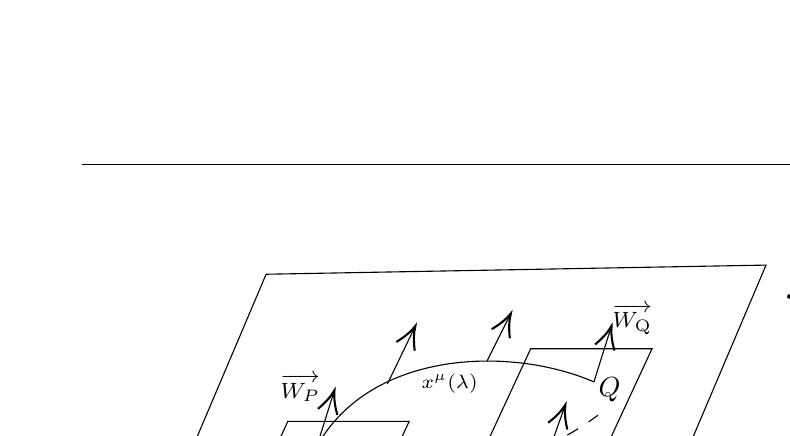
\begin{tikzpicture}[x=0.75pt,y=0.75pt,yscale=-1,xscale=1]
                %uncomment if require: \path (0,300); %set diagram left start at 0, and has height of 300
                
                %Shape: Parallelogram [id:dp45686716922248394] 
                \draw   (188.57,57.12) -- (429.42,52.71) -- (354.35,229.59) -- (113.5,234) -- cycle ;
                %Shape: Parallelogram [id:dp49694338363773927] 
                \draw   (199.05,128) -- (257.5,128) -- (232.45,182) -- (174,182) -- cycle ;
                %Shape: Parallelogram [id:dp3574677645623825] 
                \draw   (316.05,93) -- (374.5,93) -- (349.45,147) -- (291,147) -- cycle ;
                %Straight Lines [id:da8246844143539966] 
                \draw    (164.5,211) -- (188.06,188.39) ;
                \draw [shift={(189.5,187)}, rotate = 496.17] [color={rgb, 255:red, 0; green, 0; blue, 0 }  ][line width=0.75]    (10.93,-3.29) .. controls (6.95,-1.4) and (3.31,-0.3) .. (0,0) .. controls (3.31,0.3) and (6.95,1.4) .. (10.93,3.29)   ;
                %Straight Lines [id:da5664491078672309] 
                \draw    (402.5,184) -- (363.81,139.51) ;
                \draw [shift={(362.5,138)}, rotate = 408.99] [color={rgb, 255:red, 0; green, 0; blue, 0 }  ][line width=0.75]    (10.93,-3.29) .. controls (6.95,-1.4) and (3.31,-0.3) .. (0,0) .. controls (3.31,0.3) and (6.95,1.4) .. (10.93,3.29)   ;
                %Curve Lines [id:da23513303708004218] 
                \draw    (213,140) .. controls (239.5,93) and (307.5,92) .. (346.5,109) ;
                %Curve Lines [id:da5246984843004461] 
                \draw  [dash pattern={on 4.5pt off 4.5pt}]  (207.5,151) .. controls (236.25,170) and (308.5,155) .. (348.5,125) ;
                %Straight Lines [id:da48389451560387475] 
                \draw    (213,140) -- (220.9,114.91) ;
                \draw [shift={(221.5,113)}, rotate = 467.47] [color={rgb, 255:red, 0; green, 0; blue, 0 }  ][line width=0.75]    (10.93,-4.9) .. controls (6.95,-2.3) and (3.31,-0.67) .. (0,0) .. controls (3.31,0.67) and (6.95,2.3) .. (10.93,4.9)   ;
                %Straight Lines [id:da8163241029539516] 
                \draw    (247,110) -- (259.63,83.8) ;
                \draw [shift={(260.5,82)}, rotate = 475.74] [color={rgb, 255:red, 0; green, 0; blue, 0 }  ][line width=0.75]    (10.93,-4.9) .. controls (6.95,-2.3) and (3.31,-0.67) .. (0,0) .. controls (3.31,0.67) and (6.95,2.3) .. (10.93,4.9)   ;
                %Straight Lines [id:da7307279955715706] 
                \draw    (295,99) -- (305.61,77.79) ;
                \draw [shift={(306.5,76)}, rotate = 476.57] [color={rgb, 255:red, 0; green, 0; blue, 0 }  ][line width=0.75]    (10.93,-4.9) .. controls (6.95,-2.3) and (3.31,-0.67) .. (0,0) .. controls (3.31,0.67) and (6.95,2.3) .. (10.93,4.9)   ;
                %Straight Lines [id:da8511921182852662] 
                \draw    (346.5,109) -- (354.4,83.91) ;
                \draw [shift={(355,82)}, rotate = 467.47] [color={rgb, 255:red, 0; green, 0; blue, 0 }  ][line width=0.75]    (10.93,-4.9) .. controls (6.95,-2.3) and (3.31,-0.67) .. (0,0) .. controls (3.31,0.67) and (6.95,2.3) .. (10.93,4.9)   ;
                %Straight Lines [id:da4582888124741773] 
                \draw    (215.75,155) -- (225.33,141.63) ;
                \draw [shift={(226.5,140)}, rotate = 485.63] [color={rgb, 255:red, 0; green, 0; blue, 0 }  ][line width=0.75]    (10.93,-4.9) .. controls (6.95,-2.3) and (3.31,-0.67) .. (0,0) .. controls (3.31,0.67) and (6.95,2.3) .. (10.93,4.9)   ;
                %Straight Lines [id:da1540386691479012] 
                \draw    (245,159) -- (255.33,144.62) ;
                \draw [shift={(256.5,143)}, rotate = 485.71] [color={rgb, 255:red, 0; green, 0; blue, 0 }  ][line width=0.75]    (10.93,-4.9) .. controls (6.95,-2.3) and (3.31,-0.67) .. (0,0) .. controls (3.31,0.67) and (6.95,2.3) .. (10.93,4.9)   ;
                %Straight Lines [id:da26032488069998605] 
                \draw    (283,155) -- (287.88,139.9) ;
                \draw [shift={(288.5,138)}, rotate = 467.93] [color={rgb, 255:red, 0; green, 0; blue, 0 }  ][line width=0.75]    (10.93,-4.9) .. controls (6.95,-2.3) and (3.31,-0.67) .. (0,0) .. controls (3.31,0.67) and (6.95,2.3) .. (10.93,4.9)   ;
                %Straight Lines [id:da5859608433627239] 
                \draw    (326,139) -- (332.08,121.88) ;
                \draw [shift={(332.75,120)}, rotate = 469.56] [color={rgb, 255:red, 0; green, 0; blue, 0 }  ][line width=0.75]    (10.93,-4.9) .. controls (6.95,-2.3) and (3.31,-0.67) .. (0,0) .. controls (3.31,0.67) and (6.95,2.3) .. (10.93,4.9)   ;
                
                % Text Node
                \draw (205.75,142) node    {$P$};
                % Text Node
                \draw (354,113) node    {$Q$};
                % Text Node
                \draw (418,189) node    {$T_{Q}$};
                % Text Node
                \draw (157,212) node    {$T_{P}$};
                % Text Node
                \draw (451,62) node  [font=\Large]  {$\mathcal{{\displaystyle M}}$};
                % Text Node
                \draw (277,110) node  [font=\scriptsize]  {$x^{\mu }( \lambda )$};
                % Text Node
                \draw (205,112) node  [font=\footnotesize]  {$\overrightarrow{W_{P}}$};
                % Text Node
                \draw (365,79) node  [font=\footnotesize]  {$\overrightarrow{W_{\text{Q}}}$};
                
                
                \end{tikzpicture}
                
         \caption{The parallel transport of $\vec W$ along $x^\mu$ to some transported $\vec W$ at point $Q$.}       
	\end{center}
        \end{figure}
    
    In order to parallel transport we choose a curve parametrized by $\lambda$,  $x^\mu (\lambda)$ with a tangent given by $V^\mu = \frac{d x^\mu}{d\lambda}$. The equation  
    \begin{align}
    \nabla_{\vec V} \vec W=V^\beta \left( \partial_\beta W ^\mu + \Gamma^\mu_{\beta \alpha} W^\alpha \right) = 0,
    \end{align}
    
    defines the parallel transport with respect to a given connection. This boils down to a set of $1^{\text{st}}$ order ODEs for the components of $\vec W$ with $\vec W^\mu|_p$ as the initial conditions. 
    
    Different connections define different rules of parallel transport -- or how to keep a vector the 'same' during transport. Generally the solution given by parallel transport will be path dependent, unless however the curvature vanishes. This can be seen in the figure below. \begin{figure}[h]
    \begin{center}
                        
                    
                    \tikzset{every picture/.style={line width=0.75pt}} %set default line width to 0.75pt        
                    
                    \begin{tikzpicture}[x=0.75pt,y=0.75pt,yscale=-1,xscale=1]
                    %uncomment if require: \path (0,300); %set diagram left start at 0, and has height of 300
                    
                    %Curve Lines [id:da7970850461973555] 
                    \draw    (101,184) .. controls (149.5,110) and (253.5,124) .. (284.5,214) ;
                    %Curve Lines [id:da6353765339785125] 
                    \draw    (101,184) .. controls (104.5,239) and (214.5,279) .. (284.5,214) ;
                    %Straight Lines [id:da05837049859307886] 
                    \draw    (101,184) -- (90.01,141.94) ;
                    \draw [shift={(89.5,140)}, rotate = 435.35] [color={rgb, 255:red, 0; green, 0; blue, 0 }  ][line width=0.75]    (10.93,-3.29) .. controls (6.95,-1.4) and (3.31,-0.3) .. (0,0) .. controls (3.31,0.3) and (6.95,1.4) .. (10.93,3.29)   ;
                    %Straight Lines [id:da13780093371010316] 
                    \draw    (134,151) -- (123.01,108.94) ;
                    \draw [shift={(122.5,107)}, rotate = 435.35] [color={rgb, 255:red, 0; green, 0; blue, 0 }  ][line width=0.75]    (10.93,-3.29) .. controls (6.95,-1.4) and (3.31,-0.3) .. (0,0) .. controls (3.31,0.3) and (6.95,1.4) .. (10.93,3.29)   ;
                    %Straight Lines [id:da10130628868499003] 
                    \draw    (188,136) -- (188.48,97) ;
                    \draw [shift={(188.5,95)}, rotate = 450.7] [color={rgb, 255:red, 0; green, 0; blue, 0 }  ][line width=0.75]    (10.93,-3.29) .. controls (6.95,-1.4) and (3.31,-0.3) .. (0,0) .. controls (3.31,0.3) and (6.95,1.4) .. (10.93,3.29)   ;
                    %Straight Lines [id:da153008088853271] 
                    \draw    (231,148) -- (232.43,108) ;
                    \draw [shift={(232.5,106)}, rotate = 452.05] [color={rgb, 255:red, 0; green, 0; blue, 0 }  ][line width=0.75]    (10.93,-3.29) .. controls (6.95,-1.4) and (3.31,-0.3) .. (0,0) .. controls (3.31,0.3) and (6.95,1.4) .. (10.93,3.29)   ;
                    %Straight Lines [id:da5838899593015612] 
                    \draw    (261,172) -- (273.85,134.89) ;
                    \draw [shift={(274.5,133)}, rotate = 469.09] [color={rgb, 255:red, 0; green, 0; blue, 0 }  ][line width=0.75]    (10.93,-3.29) .. controls (6.95,-1.4) and (3.31,-0.3) .. (0,0) .. controls (3.31,0.3) and (6.95,1.4) .. (10.93,3.29)   ;
                    %Straight Lines [id:da1964119035999332] 
                    \draw    (284.5,214) -- (300.76,172.86) ;
                    \draw [shift={(301.5,171)}, rotate = 471.57] [color={rgb, 255:red, 0; green, 0; blue, 0 }  ][line width=0.75]    (10.93,-3.29) .. controls (6.95,-1.4) and (3.31,-0.3) .. (0,0) .. controls (3.31,0.3) and (6.95,1.4) .. (10.93,3.29)   ;
                    %Straight Lines [id:da7919367650778628] 
                    \draw    (127,227) -- (116.01,184.94) ;
                    \draw [shift={(115.5,183)}, rotate = 435.35] [color={rgb, 255:red, 0; green, 0; blue, 0 }  ][line width=0.75]    (10.93,-3.29) .. controls (6.95,-1.4) and (3.31,-0.3) .. (0,0) .. controls (3.31,0.3) and (6.95,1.4) .. (10.93,3.29)   ;
                    %Straight Lines [id:da09186267208805732] 
                    \draw    (176,245) -- (165.01,202.94) ;
                    \draw [shift={(164.5,201)}, rotate = 435.35] [color={rgb, 255:red, 0; green, 0; blue, 0 }  ][line width=0.75]    (10.93,-3.29) .. controls (6.95,-1.4) and (3.31,-0.3) .. (0,0) .. controls (3.31,0.3) and (6.95,1.4) .. (10.93,3.29)   ;
                    %Straight Lines [id:da9572453492531723] 
                    \draw    (227,245) -- (216.01,202.94) ;
                    \draw [shift={(215.5,201)}, rotate = 435.35] [color={rgb, 255:red, 0; green, 0; blue, 0 }  ][line width=0.75]    (10.93,-3.29) .. controls (6.95,-1.4) and (3.31,-0.3) .. (0,0) .. controls (3.31,0.3) and (6.95,1.4) .. (10.93,3.29)   ;
                    %Straight Lines [id:da3068748754885948] 
                    \draw    (273,223) -- (262.01,180.94) ;
                    \draw [shift={(261.5,179)}, rotate = 435.35] [color={rgb, 255:red, 0; green, 0; blue, 0 }  ][line width=0.75]    (10.93,-3.29) .. controls (6.95,-1.4) and (3.31,-0.3) .. (0,0) .. controls (3.31,0.3) and (6.95,1.4) .. (10.93,3.29)   ;
                    %Straight Lines [id:da45017798156811883] 
                    \draw    (284.5,214) -- (273.51,171.94) ;
                    \draw [shift={(273,170)}, rotate = 435.35] [color={rgb, 255:red, 0; green, 0; blue, 0 }  ][line width=0.75]    (10.93,-3.29) .. controls (6.95,-1.4) and (3.31,-0.3) .. (0,0) .. controls (3.31,0.3) and (6.95,1.4) .. (10.93,3.29)   ;
                    %Curve Lines [id:da14412398495524337] 
                    \draw    (356.5,136) .. controls (314.92,160.75) and (371.35,159.04) .. (306.5,191.02) ;
                    \draw [shift={(304.5,192)}, rotate = 334.11] [fill={rgb, 255:red, 0; green, 0; blue, 0 }  ][line width=0.08]  [draw opacity=0] (8.93,-4.29) -- (0,0) -- (8.93,4.29) -- cycle    ;
                    %Curve Lines [id:da601105711627504] 
                    \draw    (288.5,86) .. controls (247.34,110.5) and (307.02,135.96) .. (284.01,176.5) ;
                    \draw [shift={(282.5,179)}, rotate = 302.74] [fill={rgb, 255:red, 0; green, 0; blue, 0 }  ][line width=0.08]  [draw opacity=0] (8.93,-4.29) -- (0,0) -- (8.93,4.29) -- cycle    ;
                    
                    % Text Node
                    \draw (76,165) node    {$\vec{W}$};
                    % Text Node
                    \draw (346,120) node    {$\vec{W} \ \text{along 2}$};
                    % Text Node
                    \draw (312,70) node    {$\vec{W} \ \text{along 1}$};
                    
                    
                    \end{tikzpicture}
                    \caption{The parallel transport of $\vec W$ along two different curves will generally not result in the same transported vector.}
    	\end{center}
    \end{figure}
    
%
%    \begin{figure}
%    \begin{center}
%                        
%                    \tikzset{every picture/.style={line width=0.5pt}} %set default line width to 0.75pt        
%                    
%                    \begin{tikzpicture}[x=0.75pt,y=0.75pt,yscale=-1,xscale=1]
%                    %uncomment if require: \path (0,300); %set diagram left start at 0, and has height of 300
%                    
%                    %Curve Lines [id:da6439402381515371] 
%                    \draw    (71.5,198) .. controls (74.5,198) and (169.5,263) .. (300.5,201) ;
%                    %Straight Lines [id:da004649770794803665] 
%                    \draw    (71.5,198) -- (74.41,133) ;
%                    \draw [shift={(74.5,131)}, rotate = 452.56] [color={rgb, 255:red, 0; green, 0; blue, 0 }  ][line width=0.75]    (10.93,-3.29) .. controls (6.95,-1.4) and (3.31,-0.3) .. (0,0) .. controls (3.31,0.3) and (6.95,1.4) .. (10.93,3.29)   ;
%                    %Straight Lines [id:da04642691208090155] 
%                    \draw    (300.5,201) -- (303.41,136) ;
%                    \draw [shift={(303.5,134)}, rotate = 452.56] [color={rgb, 255:red, 0; green, 0; blue, 0 }  ][line width=0.75]    (10.93,-3.29) .. controls (6.95,-1.4) and (3.31,-0.3) .. (0,0) .. controls (3.31,0.3) and (6.95,1.4) .. (10.93,3.29)   ;
%                    %Straight Lines [id:da5852930630109445] 
%                    \draw    (300.5,201) -- (337.38,146.65) ;
%                    \draw [shift={(338.5,145)}, rotate = 484.16] [color={rgb, 255:red, 0; green, 0; blue, 0 }  ][line width=0.75]    (10.93,-3.29) .. controls (6.95,-1.4) and (3.31,-0.3) .. (0,0) .. controls (3.31,0.3) and (6.95,1.4) .. (10.93,3.29)   ;
%                    %Straight Lines [id:da5898447173086896] 
%                    \draw    (93.5,143) -- (281.5,141.02) ;
%                    \draw [shift={(283.5,141)}, rotate = 539.4] [color={rgb, 255:red, 0; green, 0; blue, 0 }  ][line width=0.75]    (10.93,-3.29) .. controls (6.95,-1.4) and (3.31,-0.3) .. (0,0) .. controls (3.31,0.3) and (6.95,1.4) .. (10.93,3.29)   ;
%                    
%                    % Text Node
%                    \draw (181,210) node  [font=\large]  {$\epsilon $};
%                    % Text Node
%                    \draw (62,208) node    {$P$};
%                    % Text Node
%                    \draw (307,208) node    {$Q$};
%                    % Text Node
%                    \draw (99,127) node  [font=\small]  {$W^{\mu }( P)$};
%                    % Text Node
%                    \draw (362,164) node  [font=\small]  {$W^{\mu }( Q)$};
%                    % Text Node
%                    \draw (305,121) node  [font=\small]  {$W^{\mu }_{\text{transported}}$};
%                    
%                    
%                    \end{tikzpicture}
%                                        
%    \end{center}
%    \end{figure}
    
       For two vectors $\vec A$ and $\vec B$, we can show that under any metric compatible covariant derivative the parallel transport of the vectors will preserve the inner product (angle)  between them. For the parallel transported vectors we have  $\nabla_{\vec V} \vec A = 0$ and $\nabla_{\vec V} \vec B=0$. The angle between $\vec A$ and $\vec B$ is defined as 
    \begin{align}
	A^\mu B^\nu g_{\mu \nu} = A^\mu B_\mu = \text{"angle"}.  
	\end{align}
	Now computing the parallel transport along their inner product we find 
\begin{align}
	\nabla_{\vec V} \left( A^\mu B_\mu \right) = A^\mu B^\nu \nabla_{\vec V} (g_{\mu \nu}) + A^\mu g_{\mu \nu} \nabla_{\vec V} B^\nu + A^\nu g_{\mu \nu} \nabla_{\vec V} B^\mu =0
    \end{align}

  \begin{figure}[h]   
    \begin{center}
 
                \tikzset{every picture/.style={line width=0.5pt}} %set default line width to 0.75pt        
                
                \begin{tikzpicture}[x=0.75pt,y=0.75pt,yscale=-1,xscale=1]
                %uncomment if require: \path (0,300); %set diagram left start at 0, and has height of 300
                
                %Curve Lines [id:da9570276194239729] 
                \draw    (140,122) .. controls (179.5,54) and (388.5,219) .. (454.5,121) ;
                %Straight Lines [id:da7016830486075938] 
                \draw    (141,120) -- (120.25,68.85) ;
                \draw [shift={(119.5,67)}, rotate = 427.91999999999996] [color={rgb, 255:red, 0; green, 0; blue, 0 }  ][line width=0.75]    (10.93,-3.29) .. controls (6.95,-1.4) and (3.31,-0.3) .. (0,0) .. controls (3.31,0.3) and (6.95,1.4) .. (10.93,3.29)   ;
                %Straight Lines [id:da3446611304914631] 
                \draw    (141,120) -- (149.21,63.98) ;
                \draw [shift={(149.5,62)}, rotate = 458.34] [color={rgb, 255:red, 0; green, 0; blue, 0 }  ][line width=0.75]    (10.93,-3.29) .. controls (6.95,-1.4) and (3.31,-0.3) .. (0,0) .. controls (3.31,0.3) and (6.95,1.4) .. (10.93,3.29)   ;
                %Straight Lines [id:da5217484020196854] 
                \draw    (425,145) -- (404.25,93.85) ;
                \draw [shift={(403.5,92)}, rotate = 427.91999999999996] [color={rgb, 255:red, 0; green, 0; blue, 0 }  ][line width=0.75]    (10.93,-3.29) .. controls (6.95,-1.4) and (3.31,-0.3) .. (0,0) .. controls (3.31,0.3) and (6.95,1.4) .. (10.93,3.29)   ;
                %Straight Lines [id:da12719509303118004] 
                \draw    (425,145) -- (433.21,88.98) ;
                \draw [shift={(433.5,87)}, rotate = 458.34] [color={rgb, 255:red, 0; green, 0; blue, 0 }  ][line width=0.75]    (10.93,-3.29) .. controls (6.95,-1.4) and (3.31,-0.3) .. (0,0) .. controls (3.31,0.3) and (6.95,1.4) .. (10.93,3.29)   ;
                
                % Text Node
                \draw (280,157) node    {$x^{\mu }( \lambda )$};
                % Text Node
                \draw (109,72) node  [font=\small]  {$\vec{A}$};
                % Text Node
                \draw (164,65) node  [font=\small]  {$\vec{B}$};
                % Text Node
                \draw (393,97) node  [font=\small]  {$\vec{A}$};
                % Text Node
                \draw (448,90) node  [font=\small]  {$\vec{B}$};
                
                
                \end{tikzpicture}

    
    \end{center}
    \caption{Metric compatible parallel transports preserve angles between vectors.}
    \end{figure}
    
    \section{Geodesics}
    
    We are now in the position to look at trajectories on which particle motion occurs. Consider a vector $\vec V$ which is defined as a vector parallel transported along itself. 
    \begin{figure}[h]
        \begin{center}
                        \tikzset{every picture/.style={line width=0.75pt}} %set default line width to 0.75pt        
                    
                    \begin{tikzpicture}[x=0.75pt,y=0.75pt,yscale=-1,xscale=1]
                    %uncomment if require: \path (0,300); %set diagram left start at 0, and has height of 300
                    
                    %Curve Lines [id:da197896422617873] 
                    \draw    (221,135) .. controls (261,105) and (356.5,118) .. (397.5,98) ;
                    %Straight Lines [id:da47255700142230217] 
                    \draw    (221,135) -- (255.77,115) ;
                    \draw [shift={(257.5,114)}, rotate = 510.09] [color={rgb, 255:red, 0; green, 0; blue, 0 }  ][line width=0.75]    (10.93,-3.29) .. controls (6.95,-1.4) and (3.31,-0.3) .. (0,0) .. controls (3.31,0.3) and (6.95,1.4) .. (10.93,3.29)   ;
                    %Straight Lines [id:da16635069392869717] 
                    \draw    (272,118) -- (330.51,111.23) ;
                    \draw [shift={(332.5,111)}, rotate = 533.4] [color={rgb, 255:red, 0; green, 0; blue, 0 }  ][line width=0.75]    (10.93,-3.29) .. controls (6.95,-1.4) and (3.31,-0.3) .. (0,0) .. controls (3.31,0.3) and (6.95,1.4) .. (10.93,3.29)   ;
                    %Straight Lines [id:da43701315094479787] 
                    \draw    (350,110) -- (390.54,101.41) ;
                    \draw [shift={(392.5,101)}, rotate = 528.04] [color={rgb, 255:red, 0; green, 0; blue, 0 }  ][line width=0.75]    (10.93,-3.29) .. controls (6.95,-1.4) and (3.31,-0.3) .. (0,0) .. controls (3.31,0.3) and (6.95,1.4) .. (10.93,3.29)   ;
                    
                    % Text Node
                    \draw (223,116) node    {$\vec{V}$};
                    
                    
                    \end{tikzpicture}
    
    \end{center}
    \caption{A vector $\vec V$ parallel transported along itself.}
    \end{figure}
    
    For a curve $x^\mu (\lambda)$ with tangent $V^\mu = \frac{ dx^\mu}{d\lambda}$. Then if $\nabla_{\vec V} \vec V = 0$, then the curve  $x^\mu (\lambda)$ is called a \textbf{geodesic}.  To use words  words a geodesic is a curve whose tangent is parallel transported along itself. Written out in component form, $ V^\alpha \nabla_\alpha V^\mu = 0$, which leads to the geodesic equation 
    \begin{align}
    \frac{d^2 x^\mu}{d \lambda ^2} + \Gamma^{\mu}_{\alpha \beta} \frac{dx^\alpha}{d\lambda} \frac{dx^\beta}{d\lambda} = 0
    \end{align}
    which is a $2^\text{nd}$ order ODE for the curve $x^\mu (\lambda)$ itself. Note, that sometimes the definition of a covariant derivative along a curve is written as 
    \begin{align}
    \frac{D}{d \lambda} = V^\mu \nabla_\mu = \frac{dx^\mu}{d\lambda} \nabla_\mu. 
    \end{align}
    
    In some sense this is Newton's equation written for general relativity. For gravitational forces, rather than using $F=ma$ to solve for the trajectories of particles we use $\frac{D}{d\lambda} \frac{x^\mu}{d\lambda} = 0$. Note that this will not be equal to zero but rather $\frac{F^\mu}{m}$ for non-gravitational forces where $F^\mu$ denotes the four-force and $m$ the mass of the particle.
    
    We are now in the place to define the concept of a \textbf{test particle}. A test particle is one so small that it does not influence the spacetime around it. \\ 
    \begin{minipage}{50em}
 \textit{ \quad\quad \quad\quad \quad\quad \quad\quad \quad\quad Particles in force free motion travel on geodesics}. 
\end{minipage}
    Since $\nabla_\nu$ preserves inner products on geodesics, particles will remain timelike or null on their trajectories. 
   
   \section{Symmetries}
   Before we dive into symmetries let's first take stock of all the kinds of derivatives we have. Both the exterior derivative $\undertilde{d}$ and the Lie derivative $\mathcal{L}_{\vec V}$ return tensors. For a torsion free covariant derivative we can modify both of these definitions be replacing partial derivatives with covariant derivatives. The derivatives then take the form 
   \begin{align*}
   \undertilde{d}\undertilde{\omega} &= \frac{1}{p!} \left( \nabla_\nu \omega_{\mu_1} ... d x^\nu \wedge dx^{\mu_1}\wedge...\right)\\
   \mathcal{L}_{\vec V} \vec W &= \left[ \vec V, \vec W \right] = V^\alpha \nabla_\alpha W^\mu - W^\alpha \nabla_\alpha V^\mu
   \end{align*}
   
   Given a vector $\vec K$ we take the Lie derivative of the metric 
   \begin{align}
   \left(\mathcal{L}_{\vec K} g \right)_{\mu \nu} &= K^\alpha \nabla_\alpha g_{\mu \nu} +\left( \nabla_\mu K^\alpha\right) g_{\alpha \nu} + \nabla _\nu K^\alpha g_{\alpha \mu}
   \end{align}
   The first term vanishes by metric compatibility leaving us with 
       \begin{align}
   \left(\mathcal{L}_{\vec K} g \right)_{\mu \nu} &= \nabla_\mu K_\nu + \nabla_\nu K_\mu.
   \end{align}
   
      
   If $g_{\mu \nu}$ unchanged by the Lie derivative along $\vec K$, we have a symmetry of the spacetime and can write 
   \begin{align}\label{KillingEqn}
      \mathcal{L}_{\vec K} g_{\mu \nu} = \nabla_\mu K_\nu + \nabla_\nu K_\mu= 0, 
   \end{align}
   
   where $\vec K$ is a Killing vector and \ref{KillingEqn} is known as "Killing's equation". 
   
   \begin{figure}[h]
   \begin{center}

                \tikzset{every picture/.style={line width=0.75pt}} %set default line width to 0.75pt        
                
                \begin{tikzpicture}[x=0.75pt,y=0.75pt,yscale=-1,xscale=1]
                %uncomment if require: \path (0,300); %set diagram left start at 0, and has height of 300
                
                %Shape: Rectangle [id:dp3055312217430888] 
                \draw   (188,66) -- (427.5,66) -- (427.5,187) -- (188,187) -- cycle ;
                %Straight Lines [id:da23058480467600617] 
                \draw    (219.5,90) -- (398.5,90) ;
                \draw [shift={(400.5,90)}, rotate = 180] [color={rgb, 255:red, 0; green, 0; blue, 0 }  ][line width=0.75]    (10.93,-3.29) .. controls (6.95,-1.4) and (3.31,-0.3) .. (0,0) .. controls (3.31,0.3) and (6.95,1.4) .. (10.93,3.29)   ;
                %Straight Lines [id:da12906004429010687] 
                \draw    (219.5,112) -- (398.5,112) ;
                \draw [shift={(400.5,112)}, rotate = 180] [color={rgb, 255:red, 0; green, 0; blue, 0 }  ][line width=0.75]    (10.93,-3.29) .. controls (6.95,-1.4) and (3.31,-0.3) .. (0,0) .. controls (3.31,0.3) and (6.95,1.4) .. (10.93,3.29)   ;
                %Straight Lines [id:da7227705779009779] 
                \draw    (220.5,133) -- (399.5,133) ;
                \draw [shift={(401.5,133)}, rotate = 180] [color={rgb, 255:red, 0; green, 0; blue, 0 }  ][line width=0.75]    (10.93,-3.29) .. controls (6.95,-1.4) and (3.31,-0.3) .. (0,0) .. controls (3.31,0.3) and (6.95,1.4) .. (10.93,3.29)   ;
                %Straight Lines [id:da8554229612585038] 
                \draw    (220.5,155) -- (399.5,155) ;
                \draw [shift={(401.5,155)}, rotate = 180] [color={rgb, 255:red, 0; green, 0; blue, 0 }  ][line width=0.75]    (10.93,-3.29) .. controls (6.95,-1.4) and (3.31,-0.3) .. (0,0) .. controls (3.31,0.3) and (6.95,1.4) .. (10.93,3.29)   ;
                
                % Text Node
                \draw (201,94) node    {$\vec{K}$};
                
                
                \end{tikzpicture}
                          \end{center}
                          \caption{A Killing vector field $\vec K$ that leaves a metric unchanged is a symmetry of the spacetime.}
                          \end{figure}


   
   Consider for example $\frac{dx^\mu}{d\tau} = U^\mu$ and $P^\mu = m U^\mu$, where $U^\mu$ is tangent to a geodesic. We can compute 
   \begin{align}
   U^\alpha \nabla_ \alpha \left(P_\mu K^\mu\right) &=  P_\mu U^\alpha \nabla_\alpha K^\mu+ \underbrace{\left( m U^\alpha \nabla_\alpha U_\mu\right)}_{=0 \text{ by geo. eqn.}} K^\mu \\ 
   &= m U^\alpha U^\mu \nabla_\alpha K_\nu \\&= 0
   \end{align}
   Where the last line is zero by Killing's equation. This shows that the scalar $K^\beta P_\beta$ is conserved along a geodesic for any particle.
   
   Another example is in the Schwarzschild metric $\partial_t$ is a Killing vector $\vec{\partial_t}$. 

%%%%%%%%%%%%%%%%%%%%%%%%%%%%%%%%%%%%%%%%%%
\end{document}